\documentclass[a4paper]{article}
\usepackage{latexsym,amssymb,amsmath,amsbsy,amsopn,amstext,xcolor,multicol}
\usepackage{ctex,hyperref,graphicx,wrapfig,fancybox,listings,subfigure}
\usepackage{pgf,pgfarrows,pgfnodes,pgfautomata,pgfheaps,pgfshade}
\usepackage[top=1in, bottom=1in, left=1.25in, right=1.25in]{geometry}
\graphicspath{{pic/}}
\lstset{numbers=left,
keywordstyle=\color{blue!70}, commentstyle=\color{red!50!green!50!blue!50},
frame=shadowbox,
rulesepcolor=\color{red!20!green!20!blue!20},
breaklines=true,
extendedchars=true
}
\renewcommand{\figurename}{图}
\title{\bf 数字图像处理第一次大作业报告}
\date{2018.4}
\author{计64~~翁家翌~2016011446}
\begin{document}
\kaishu
\ttfamily
\maketitle
\tableofcontents
\newpage
\section{测试环境}

本套程序在Ubuntu 14.04 LTS和Ubuntu 16.04 LTS上使用Python2/Python3均测试通过。在运行之前,请安装python的第三方包 \underline{\textbf{opencv}}和 \underline{\textbf{numpy}},使用命令
\begin{lstlisting}[language=bash]
pip install -r requirements.txt --user
\end{lstlisting}
即可安装。

\section{Point Processing}

\subsection{实现方式}

该部分仅需要读取图片中的每个点的颜色数据进行相应的处理即可。我实现了明度、对比度、Gamma 值、直方图均衡化和直方图匹配的功能。
在编程中,我使用了 Python 语言,利用 opencv 库用于图片数据的读入,并使用 numpy 库进行数组操作。

\subsection{运行说明}
只要在命令行中输入 
\begin{lstlisting}[language=bash]
./point_processing.py <args>
\end{lstlisting}
即可运行或查看帮助,如图\ref{fig:1-1}所示:
\begin{figure}[htp]
\centering
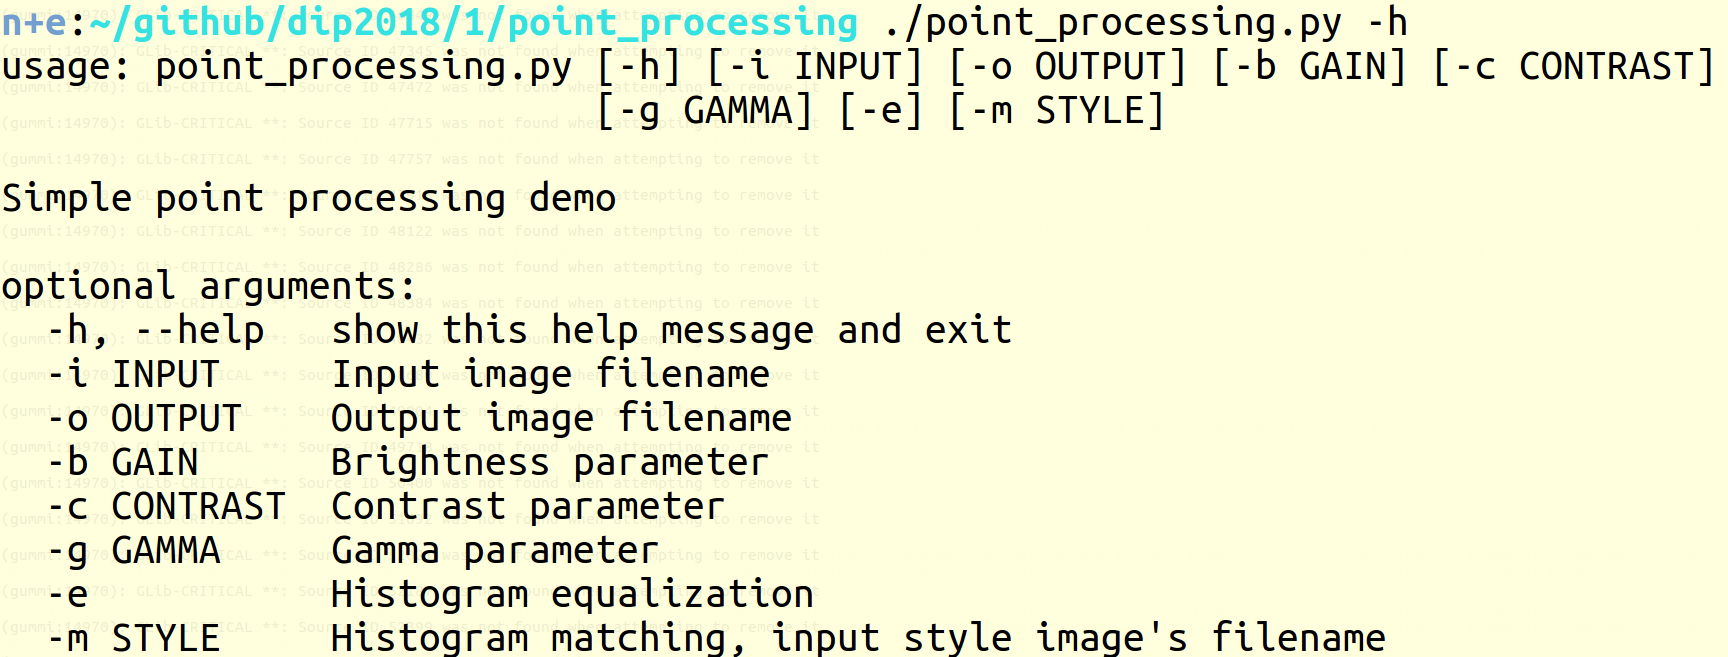
\includegraphics[width=1\linewidth]{1_1.png}
\caption{查看point\_processing帮助}
\label{fig:1-1}
\end{figure}

\subsection{实验结果}

\subsubsection{明度变化}

明度变化效果图如图\ref{fig:1-2}所示。左图增加了80明度,右图减小了80明度。

\begin{figure}[htp]
\centering
\subfigure[增加 80 明度]
{
\begin{minipage}[b]{0.45\columnwidth}
\centering
\resizebox{\columnwidth}{!}{
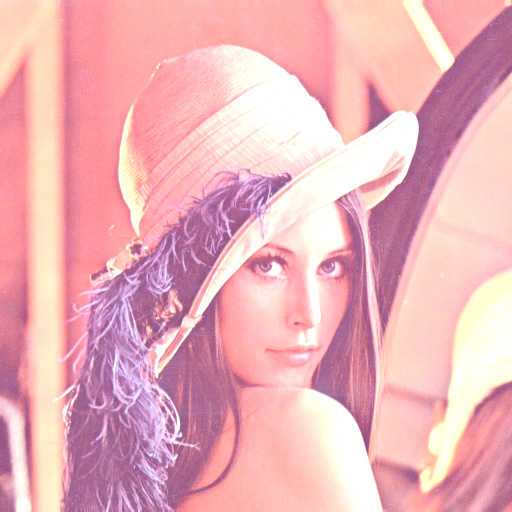
\includegraphics[width=1\columnwidth]{1_2.png} 
}
\label{fig:1-2:a}
\end{minipage}
}
\hfil
\subfigure[减小 80 明度]
{
\begin{minipage}[b]{0.45\columnwidth}
\centering
\resizebox{\columnwidth}{!}{
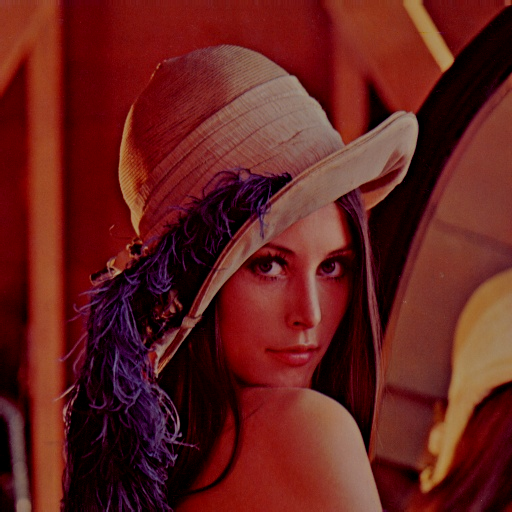
\includegraphics[width=1\columnwidth]{1_3.png}
}
\label{fig:1-2:b}
\end{minipage}
}
\caption{明度变换演示效果图}
\label{fig:1-2}
\end{figure}

\subsubsection{对比度变化}

对比度变化如图\ref{fig:1-3}所示。对比度斜率小于1则表示减小对比度,大于1表示增加对比度。

\begin{figure}[htp]
\centering
\subfigure[对比度斜率 0.5]
{
\begin{minipage}[b]{0.45\columnwidth}
\centering
\resizebox{\columnwidth}{!}{
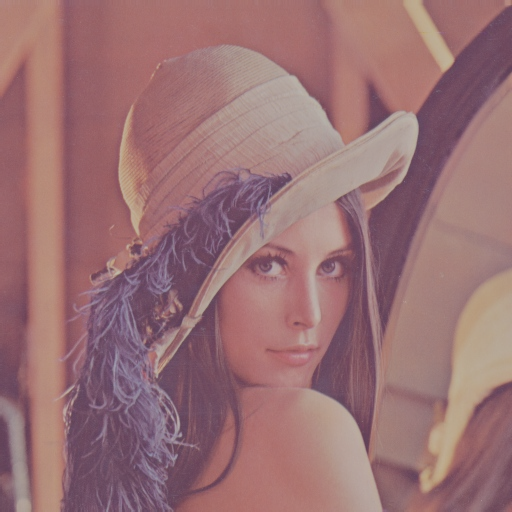
\includegraphics[width=1\columnwidth]{1_4.png} 
}
\label{fig:1-3:a}
\end{minipage}
}
\hfil
\subfigure[对比度斜率 1.5]
{
\begin{minipage}[b]{0.45\columnwidth}
\centering
\resizebox{\columnwidth}{!}{
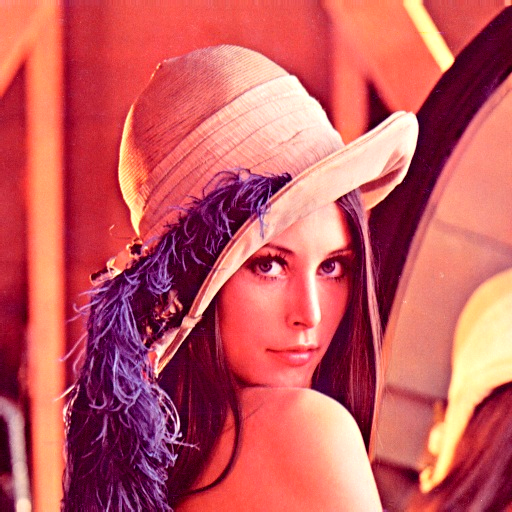
\includegraphics[width=1\columnwidth]{1_5.png}
}
\label{fig:1-3:b}
\end{minipage}
}
\caption{对比度变换演示效果图}
\label{fig:1-3}
\end{figure}

\subsubsection{Gamma 变换}

Gamma 变换如图\ref{fig:1-4}所示。当 $\gamma > 1$ 的时候图像变得更加明亮,反之图像变得更加暗淡,但是最亮处和最暗处极值处得到了保留。

\begin{figure}[htp]
\centering
\subfigure[$\gamma=0.5$]
{
\begin{minipage}[b]{0.45\columnwidth}
\centering
\resizebox{\columnwidth}{!}{
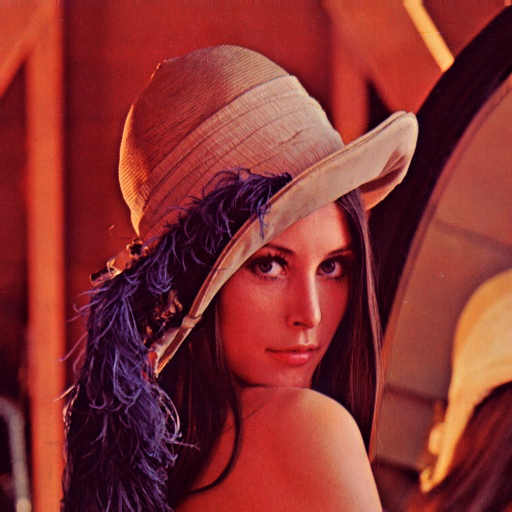
\includegraphics[width=1\columnwidth]{1_6.png} 
}
\label{fig:1-4:a}
\end{minipage}
}
\hfil
\subfigure[$\gamma=1.5$]
{
\begin{minipage}[b]{0.45\columnwidth}
\centering
\resizebox{\columnwidth}{!}{
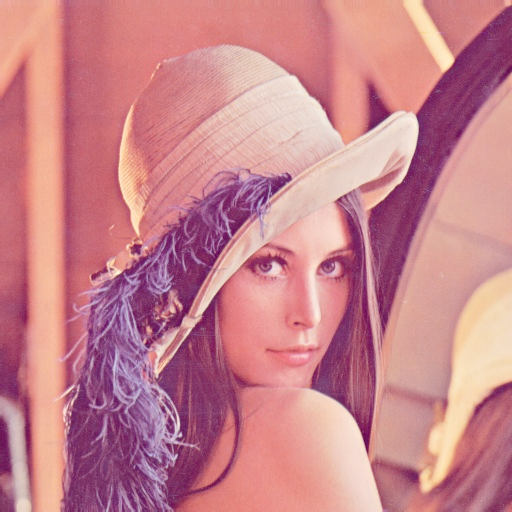
\includegraphics[width=1\columnwidth]{1_7.png}
}
\label{fig:1-4:b}
\end{minipage}
}
\caption{Gamma 变换演示效果图}
\label{fig:1-4}
\end{figure}

\subsubsection{直方图均衡化}

对于图片的每一个通道进行直方图均衡化,效果如图\ref{fig:1-5}所示。

\begin{figure}[htp]
\centering
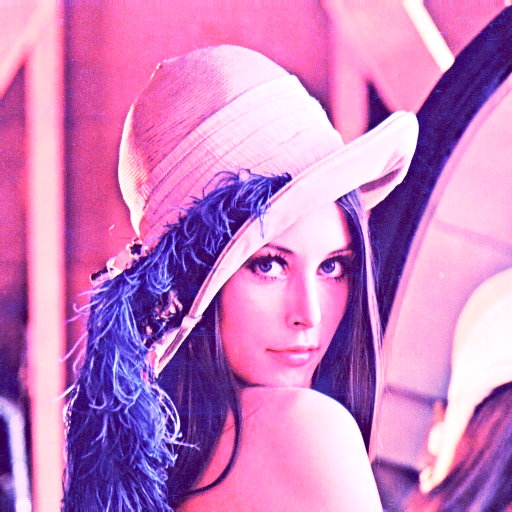
\includegraphics[width=0.45\linewidth]{1_8.png}
\caption{直方图均衡化效果图}
\label{fig:1-5}
\end{figure}

\subsubsection{直方图匹配}

我在搜狗壁纸\footnote{\url{http://bizhi.sogou.com/index.html}}中抠了几张图片下来,演示效果如图\ref{fig:1-6}所示。

\begin{figure}[htp]
\centering
\subfigure[原图]
{
\begin{minipage}[b]{0.4\columnwidth}
\centering
\resizebox{\columnwidth}{!}{
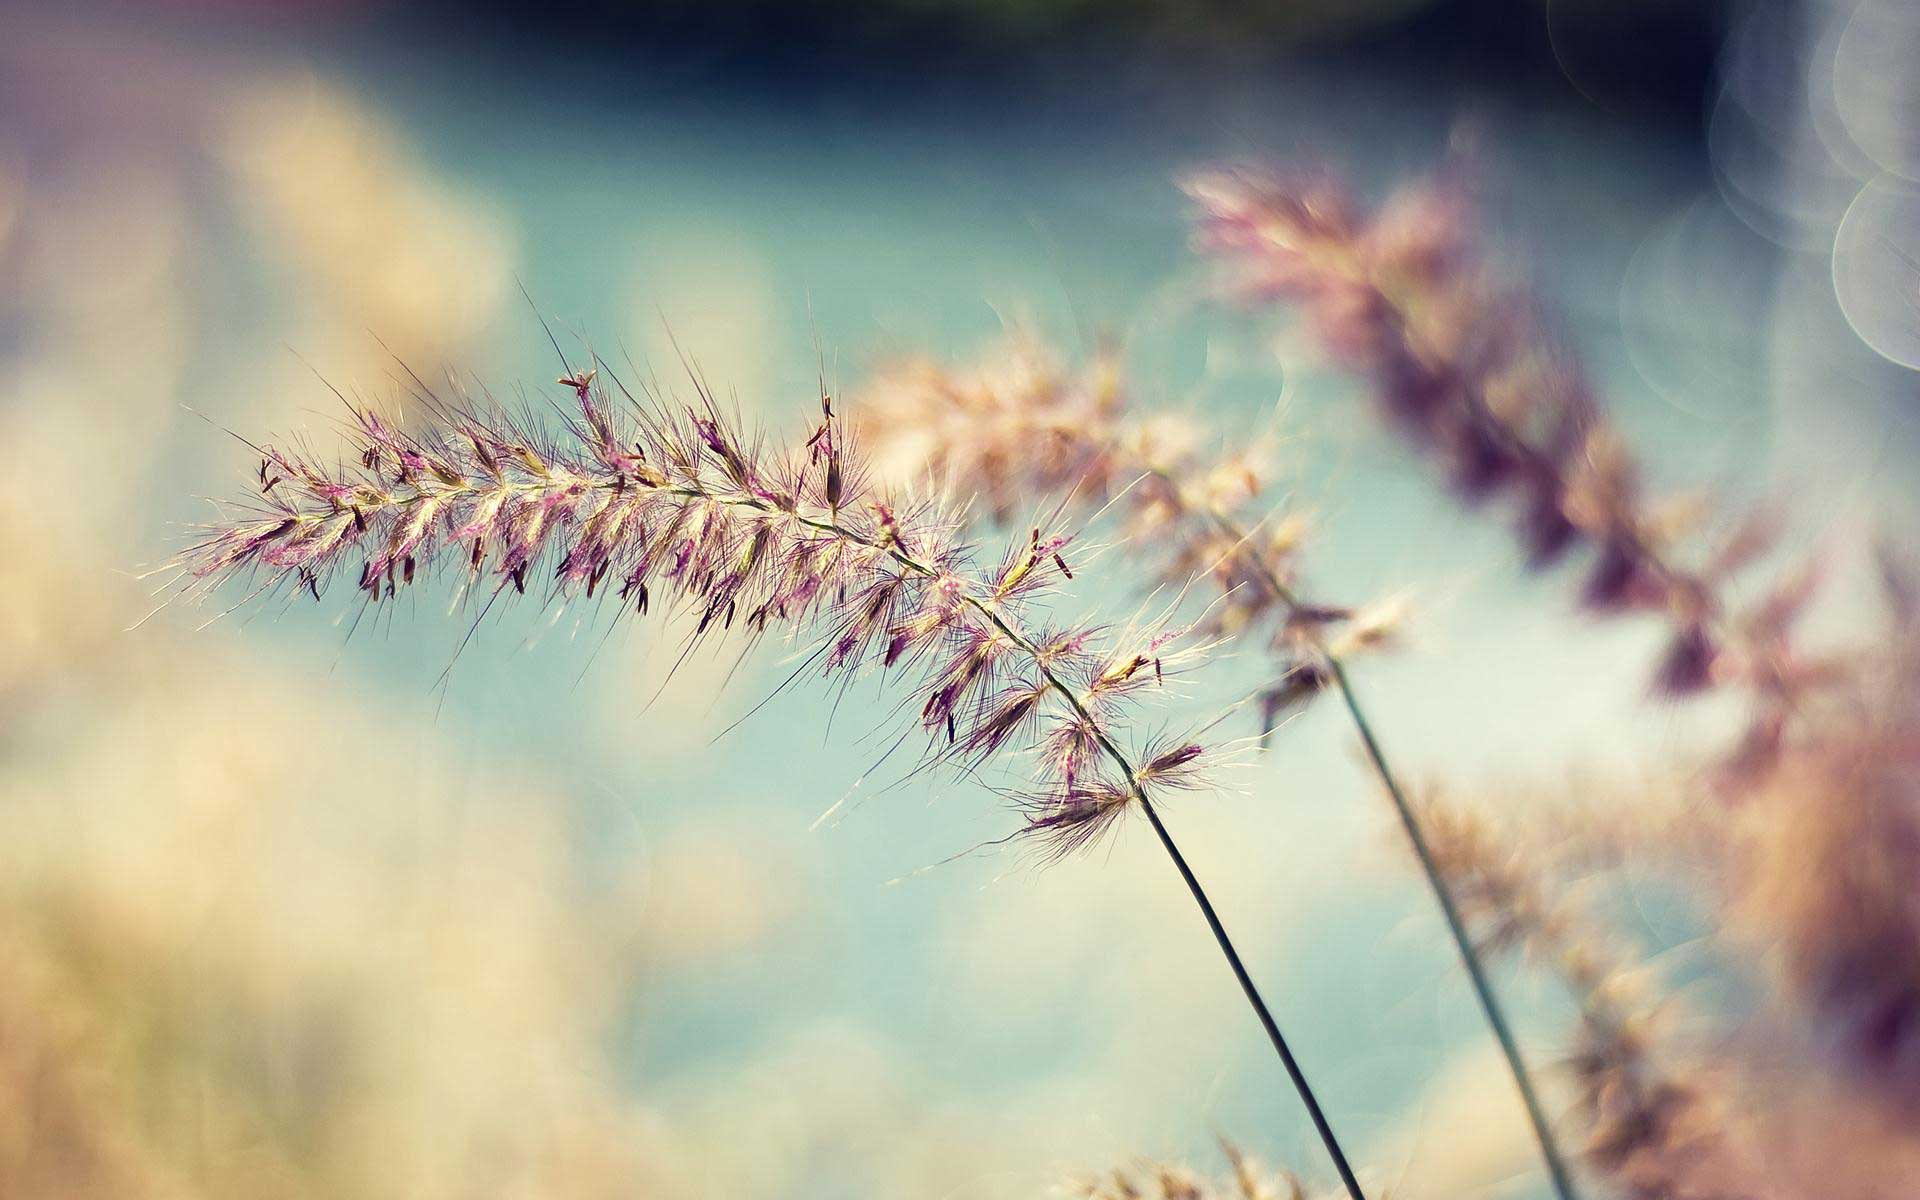
\includegraphics[width=1\columnwidth]{point_processing/image/index3_3_4.jpg} 
}
\label{fig:1-6:a}
\end{minipage}
}
\hfil
\subfigure[目标图]
{
\begin{minipage}[b]{0.5\columnwidth}
\centering
\resizebox{\columnwidth}{!}{
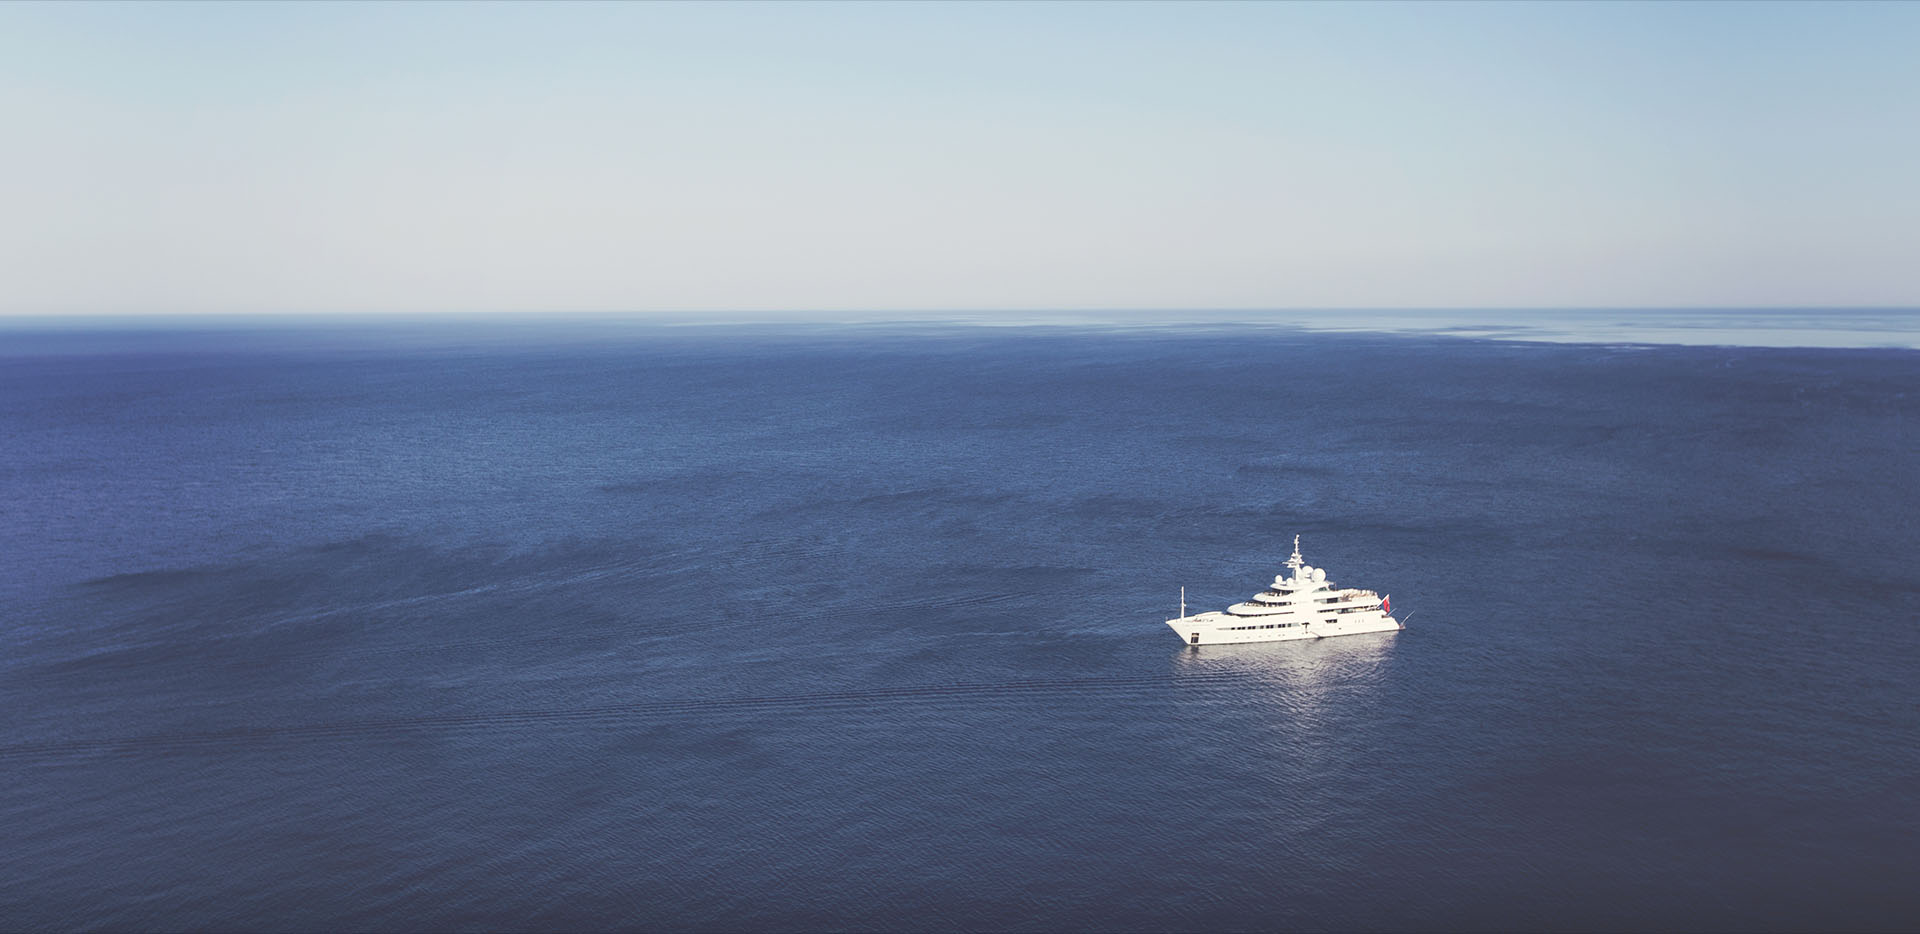
\includegraphics[width=1\columnwidth]{point_processing/image/bg1_1.jpg}
}
\label{fig:1-6:b}
\end{minipage}
}
\hfil
\subfigure[匹配结果]
{
\begin{minipage}[b]{0.6\columnwidth}
\centering
\resizebox{\columnwidth}{!}{
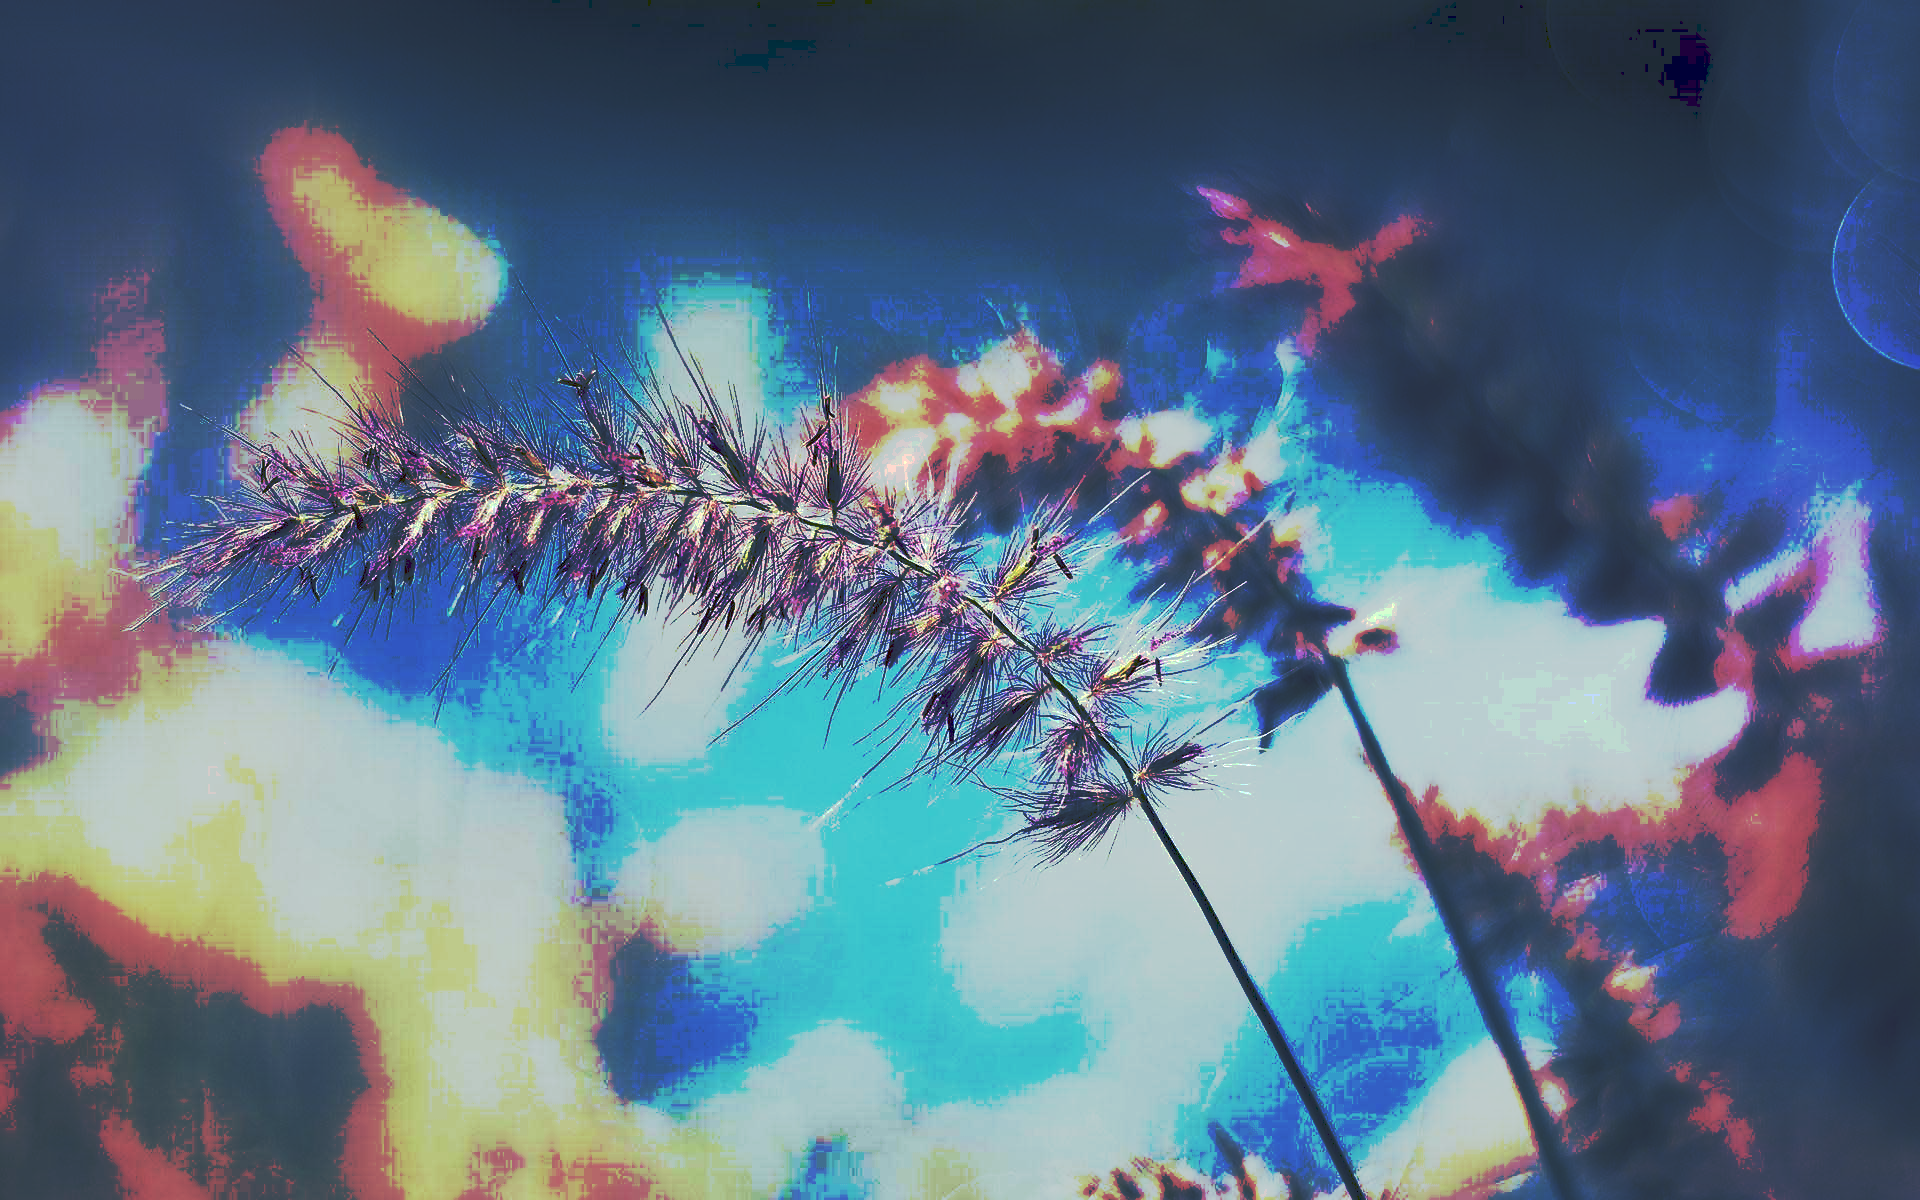
\includegraphics[width=1\columnwidth]{1_9.png}
}
\label{fig:1-6:b}
\end{minipage}
}
\caption{直方图匹配效果图}
\label{fig:1-6}
\end{figure}

\section{Image Fusion}
\subsection{实现方式}

在该部分中,考虑到实现效率,我采用C++编写代码,其中图片的读入和输出采用github上的开源仓库"stb"\footnote{\url{https://github.com/nothings/stb}}实现。

\subsection{运行说明}
首先编译C++文件:
\begin{lstlisting}[language=bash]
g++ image_fusion.cpp -o image_fusion -O2
\end{lstlisting}
在当前目录下生成可执行文件\underline{image\_fusion}。

使用命令
\begin{lstlisting}[language=bash]
./image_fusion <args>
\end{lstlisting}
即可运行或查看帮助,如图\ref{fig:2-1}所示:
\begin{figure}[htp]
\centering
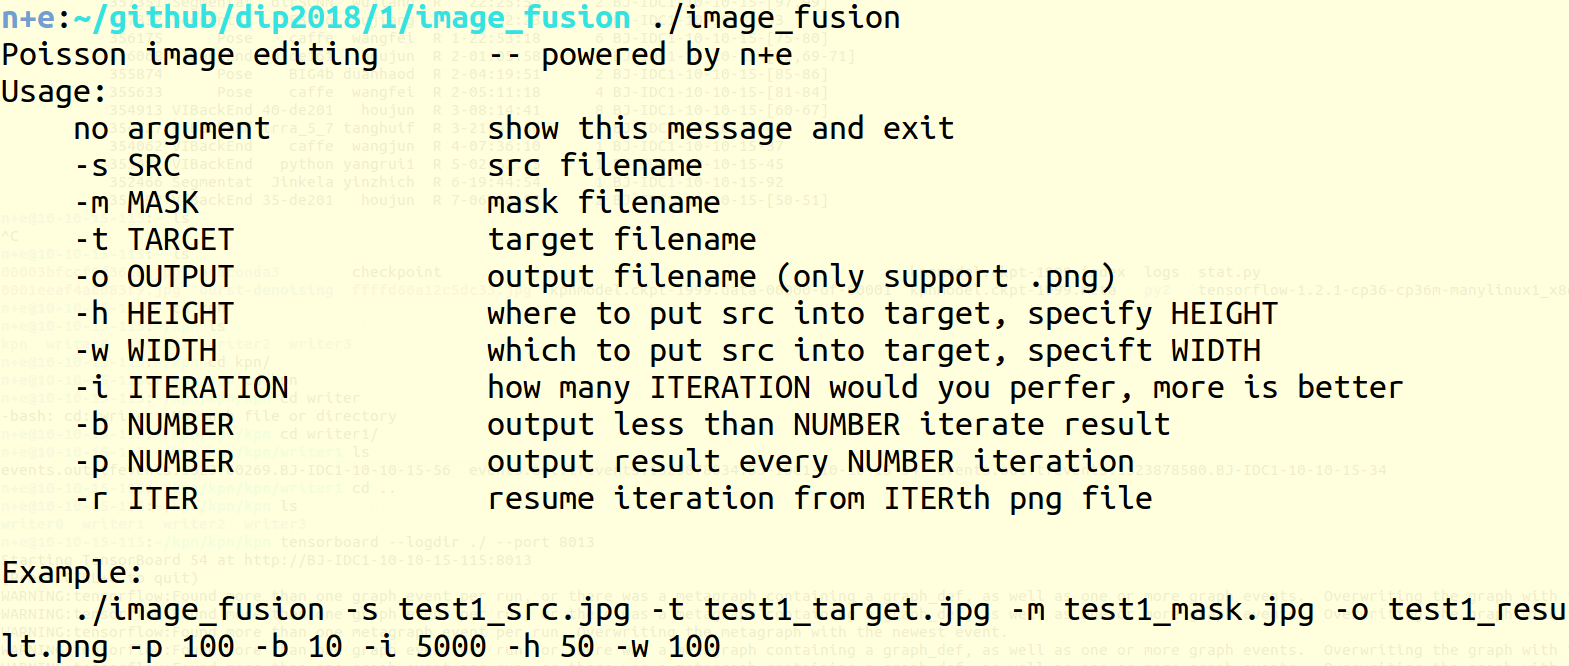
\includegraphics[width=1\linewidth]{2_1.png}
\caption{查看image\_fusion帮助}
\label{fig:2-1}
\end{figure}

\subsection{算法细节}

主体算法采用泊松图像融合算法\cite{PS,PS2},梯度计算方式为
$$
\nabla(x,y)=4I(x,y)-I(x-1,y)-I(x,y-1)-I(x+1,y)-I(x,y+1)
$$

将原图求完梯度之后,将该梯度匹配到目标图上的某一区域,本质上是一个解线性方程组的问题。形式化地,设有$N$个像素点需要匹配到目标图片中,则需要求解线性方程组
$$
A\vec{x}=\vec{b}
$$

其中$\vec{x}$代表融合后的图片中像素点的值,矩阵$A$的大小$\sim N\times N$,列向量$\vec{x}$和$\vec{b}$的大小$\sim N$,并且$A$的每一行至多只有5个非零元素,并且对角线上的元素均为4。对于第一组测试用例,$N=2150$;对于第二组测试用例,$N=16854$。因此$A$是一个巨大的稀疏矩阵。

考虑到矩阵求逆的复杂度为$O(N^3)$太高,并且某些情况下连$A$都无法直接以矩阵形式存储,因此无法直接从公式
$$
\vec{x}=A^{-1}\vec{b}
$$
求得$\vec{x}$。此处采用Jacobi Method迭代求解出$\vec{x}$的值,详见\cite{JB}。
\subsection{实验结果}
\subsubsection{Test1}
使用命令
\begin{lstlisting}[language=bash]
time ./image_fusion -s test1_src.jpg -t test1_target.jpg -m test1_mask.jpg -o test1_result.png -i 5000 -h 50 -w 100
\end{lstlisting}
可得到如下结果
\begin{lstlisting}[language=bash]
iter 5001  err 0.000000 0.000000 0.000000
real    0m0.221s
user    0m0.212s
sys     0m0.008s
\end{lstlisting}

可以看到5000轮之后误差为0,并且运行速度为0.2s左右,十分快。合成效果如图\ref{fig:2-2}所示。

\begin{figure}[htp]
\centering
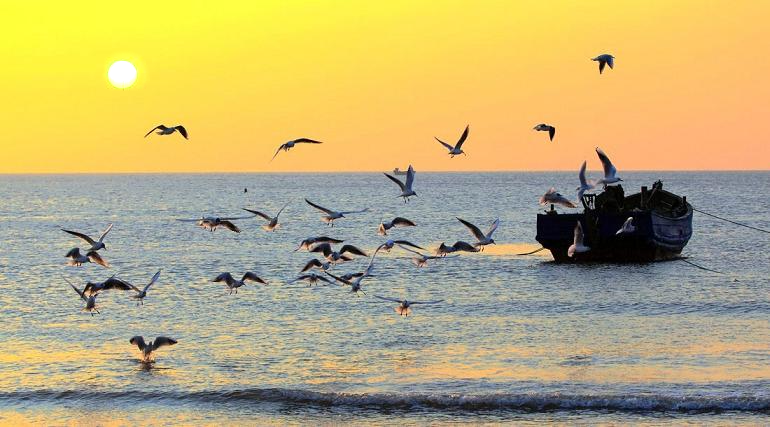
\includegraphics[width=0.8\linewidth]{2_2.png}
\caption{第一组数据合成效果}
\label{fig:2-2}
\end{figure}

动画效果见\underline{pic/test1.gif}。

\subsubsection{Test2}
使用命令
\begin{lstlisting}[language=bash]
time ./image_fusion -s test2_src.png -t test2_target.png -m test2_mask.png -o test2_result.png -i 25000 -h 150 -w 150
\end{lstlisting}
可得到如下结果
\begin{lstlisting}[language=bash]
iter 25001  err 0.000000 0.000000 0.000000
real    0m5.012s
user    0m4.992s
sys     0m0.012s
\end{lstlisting}

可以看到25000轮之后误差为0,并且运行速度为5s左右。合成效果如图\ref{fig:2-4:a}所示。

事实上,图像在几千轮迭代的时候效果并不比25000轮差,使用3000轮迭代的测试情况如下,效果如图\ref{fig:2-4:b}所示。由于我迭代的初始值选取的是目标图片的像素值,因此选用更少的迭代次数的话,合成的图片会更接近原图。

\begin{lstlisting}[language=bash]
iter 3001  err 1416.263428 842.223511 960.723694
real    0m0.677s
user    0m0.660s
sys     0m0.004s
\end{lstlisting}

\begin{figure}[htp]
\centering
\subfigure[25000轮迭代]
{
\begin{minipage}[b]{0.45\columnwidth}
\centering
\resizebox{\columnwidth}{!}{
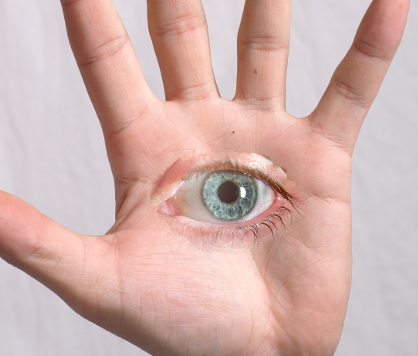
\includegraphics[width=1\columnwidth]{2_3.png} 
}
\label{fig:2-4:a}
\end{minipage}
}
\hfil
\subfigure[3000轮迭代]
{
\begin{minipage}[b]{0.45\columnwidth}
\centering
\resizebox{\columnwidth}{!}{
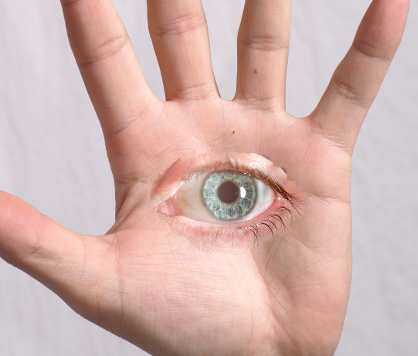
\includegraphics[width=1\columnwidth]{2_4.png}
}
\label{fig:2-4:b}
\end{minipage}
}
\caption{第二组数据合成效果}
\label{fig:2-4}
\end{figure}

动画效果见\underline{pic/test2.gif}。

\section{Face Morphing}
\subsection{实现方式}

在该部分中,考虑到实现效率,我采用C++编写核心代码,Python编写外部调用接口和JSON格式处理,主程序为merge\_traditional.py。另外,我还使用Face++的开放接口Merge Face API (V1) \footnote{\url{https://console.faceplusplus.com.cn/documents/20813963}}实现了用深度方法将两张图片进行融合,主程序为merge\_Face++.py。

\subsection{运行说明}
使用命令
\begin{lstlisting}[language=bash]
./merge_traditional <args>
\end{lstlisting}
或者
\begin{lstlisting}[language=bash]
./merge_Face++.py <args>
\end{lstlisting}
即可运行或查看帮助,如图\ref{fig:3-1}所示:
\begin{figure}[htp]
\centering
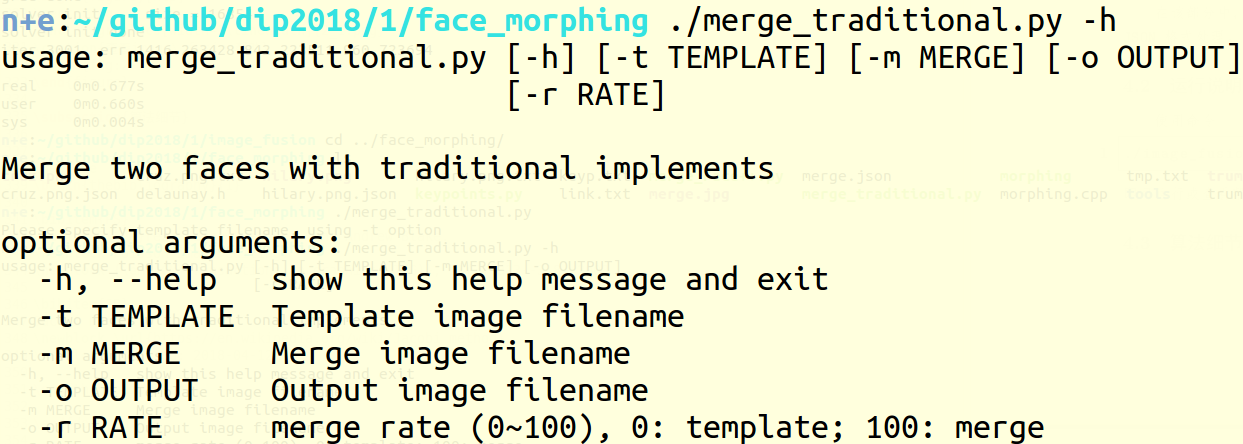
\includegraphics[width=1\linewidth]{3_1.png}
\caption{查看merge\_traditional帮助}
\label{fig:3-1}
\end{figure}

\subsection{算法细节}
此处采用Mesh-based Morphing\cite{FM},即先将图像划分成若干个三角形区域,然后将相应的三角形区域互相融合得到结果。具体而言,分为如下若干步骤:
\begin{enumerate}
	\item 获取人脸关键点坐标数据(使用Face++ Detect API V3\footnote{\url{https://console.faceplusplus.com.cn/documents/4888373}},返回 106 点人脸关键点landmark);
	\item 使用Delaunay三角剖分\cite{DT}划分图像;
	\item 对于每个三角形区域,计算仿射变换将其融合;
\end{enumerate}

根据线性代数的相关知识,考虑到仿射变换的本质是矩阵乘法,并且只要确定 Template image 的三个点和 Target image 的三个点就能建立起对应关系,如下:

$$
\begin{bmatrix}a&b&c \\ d&e&f \\ 0&0&1\end{bmatrix}
\begin{bmatrix}Temp_{1x}&Temp_{2x}&Temp_{3x}\\Temp_{1y}&Temp_{2y}&Temp_{3y}\\1&1&1\end{bmatrix}
=
\begin{bmatrix}Tar_{1x}&Tar_{2x}&Tar_{3x}\\Tar_{1y}&Tar_{2y}&Tar_{3y}\\1&1&1\end{bmatrix}
$$

其中 $$\mathcal{F}=\begin{bmatrix}a&b&c \\ d&e&f \\ 0&0&1\end{bmatrix}$$ 为仿射变换矩阵,直接用高斯消元反解方程或者矩阵求逆就能得到 $a,b,c,d,e,f$ 的值。

\subsection{实验结果}

\subsubsection{人脸关键点+Delaunay三角剖分}
三角剖分之后的可视化效果如图\ref{fig:3-2}所示。我没有按照Mallick\cite{FM}那样把耳朵、头型、衣肩、领口这些点给标出来,并且标出这些点对人脸融合的意义也不是很大。
\begin{figure}[htp]
\centering
\subfigure[Cruz]
{
\begin{minipage}[b]{0.45\columnwidth}
\centering
\resizebox{\columnwidth}{!}{
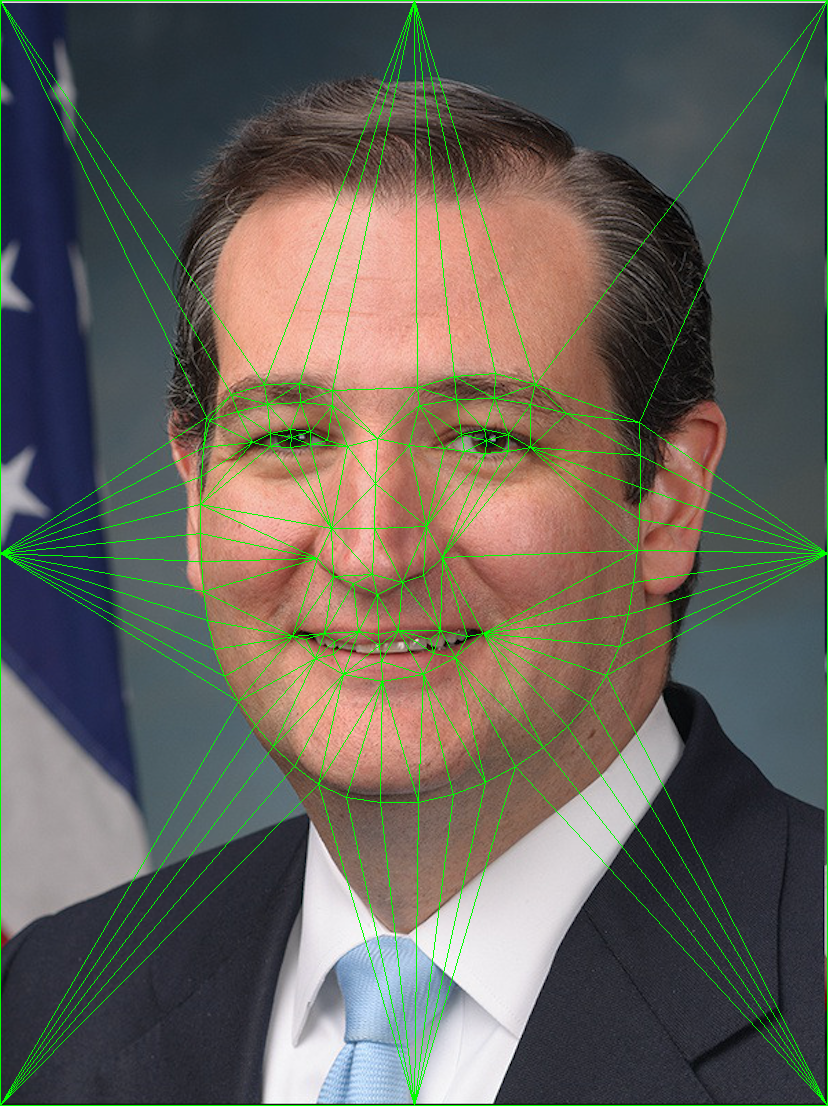
\includegraphics[width=1\columnwidth]{dt2.png}
}
\label{fig:3-2:a}
\end{minipage}
}
\hfil
\subfigure[Hillary]
{
\begin{minipage}[b]{0.45\columnwidth}
\centering
\resizebox{\columnwidth}{!}{
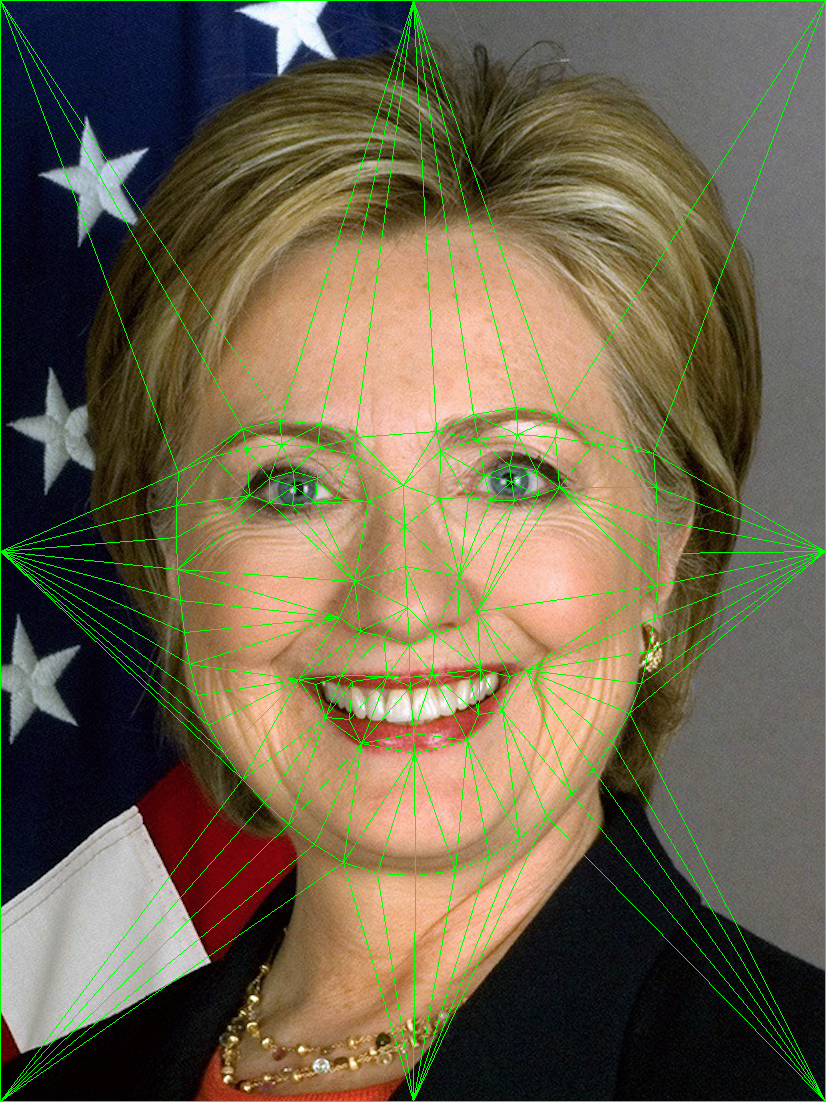
\includegraphics[width=1\columnwidth]{dt.png}
}
\label{fig:3-2:c}
\end{minipage}
}
\caption{Cruz\&Hilary的人脸三角剖分之后可视化效果}
\label{fig:3-2}
\end{figure}


\subsubsection{Cruz\&Hillary}
将Cruz和Hillary的人脸融合之后的效果如图\ref{fig:3-3}所示。合并同等规模大小的图像在本机运行的时间约为0.6s。
\begin{figure}[htp]
\centering
\subfigure[Cruz]
{
\begin{minipage}[b]{0.31\columnwidth}
\centering
\resizebox{\columnwidth}{!}{
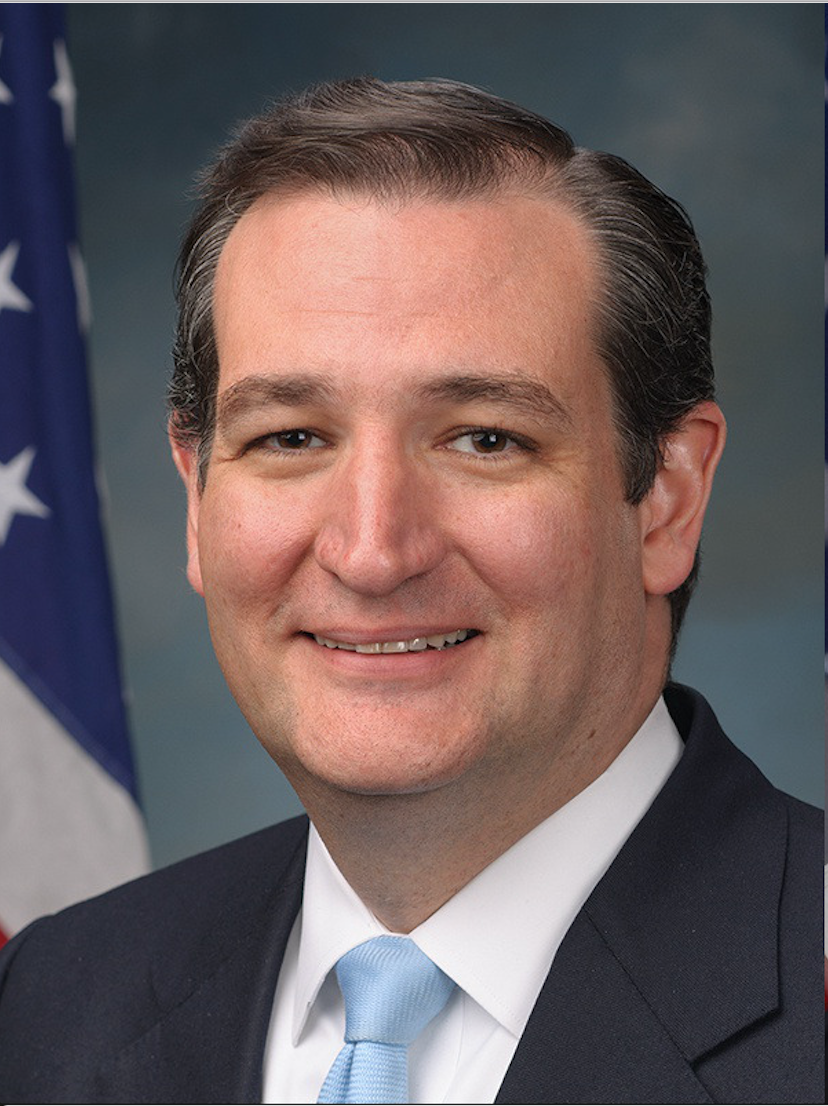
\includegraphics[width=1\columnwidth]{face_morphing/cruz.png} 
}
\label{fig:3-3:a}
\end{minipage}
}
\hfil
\subfigure[0.5C+0.5H]
{
\begin{minipage}[b]{0.31\columnwidth}
\centering
\resizebox{\columnwidth}{!}{
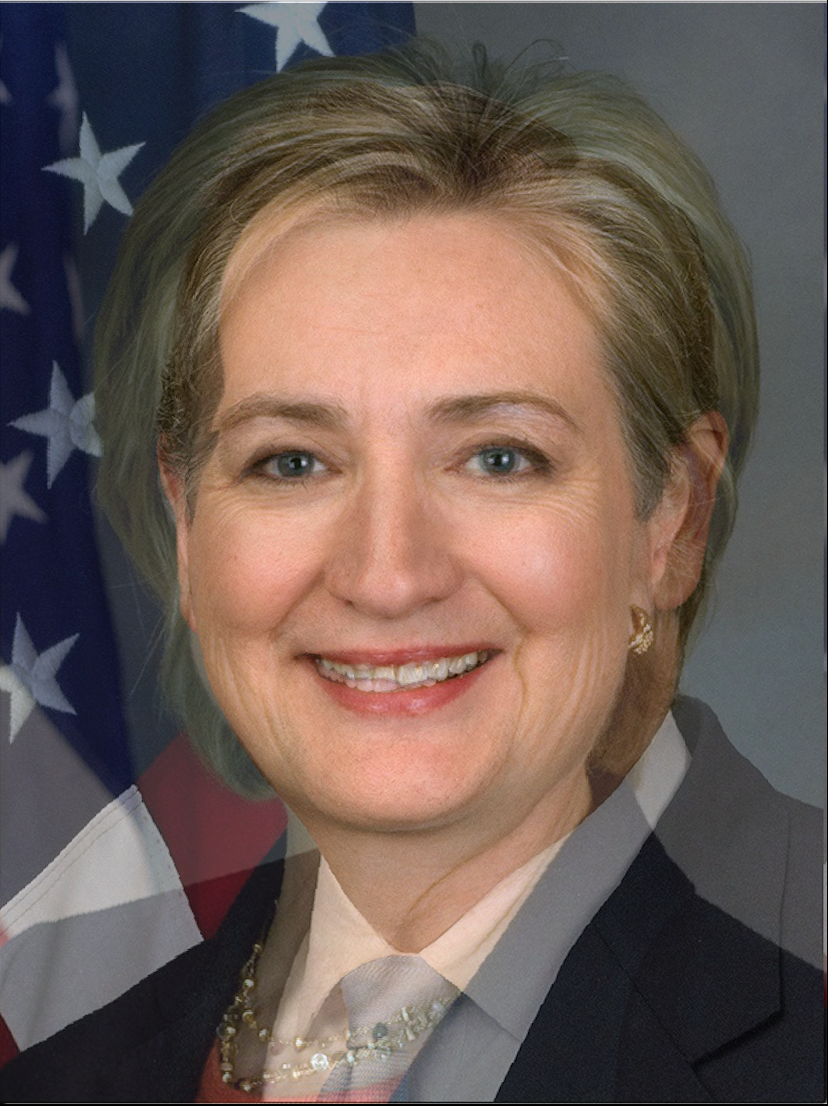
\includegraphics[width=1\columnwidth]{CH.png} 
}
\label{fig:3-3:b}
\end{minipage}
}
\hfil
\subfigure[Hillary]
{
\begin{minipage}[b]{0.31\columnwidth}
\centering
\resizebox{\columnwidth}{!}{
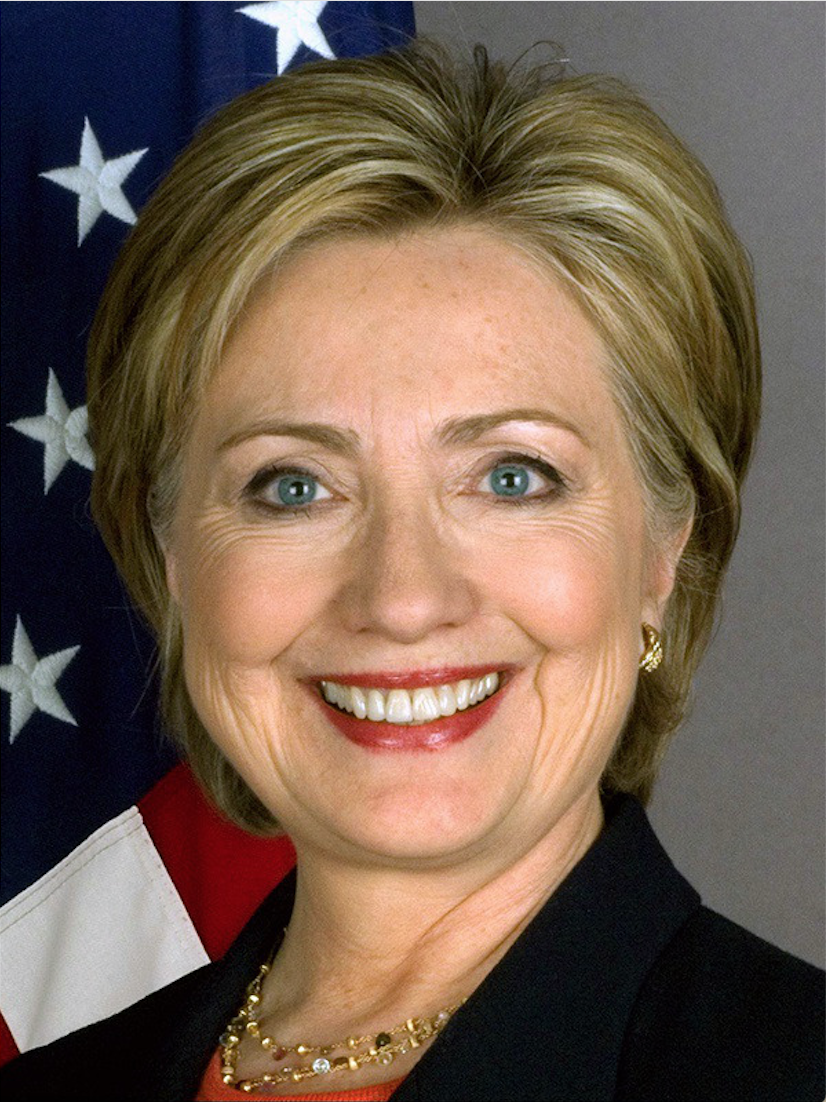
\includegraphics[width=1\columnwidth]{face_morphing/hillary.png}
}
\label{fig:3-3:c}
\end{minipage}
}
\caption{Cruz+Hilary}
\label{fig:3-3}
\end{figure}

\subsubsection{Hilary\&Trump}
将Hillary和Trump的人脸融合之后的效果如图\ref{fig:3-4}所示。
\begin{figure}[htp]
\centering
\subfigure[Hillary]
{
\begin{minipage}[b]{0.31\columnwidth}
\centering
\resizebox{\columnwidth}{!}{
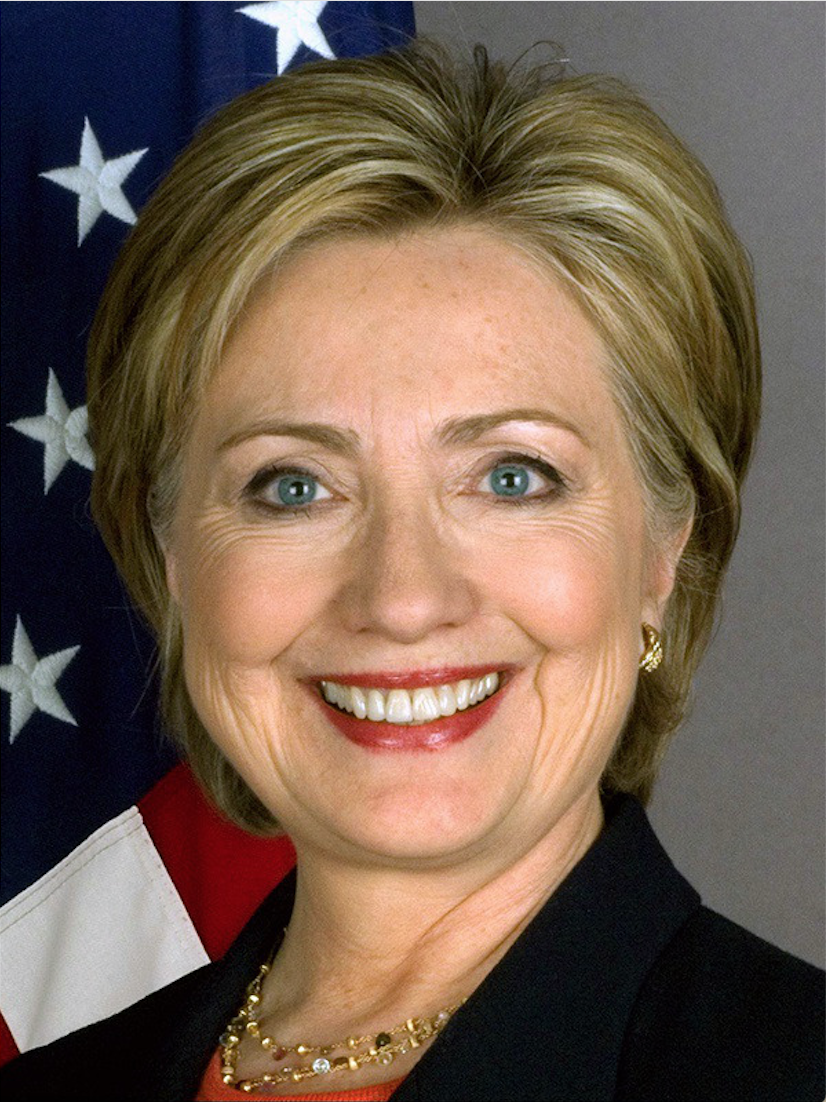
\includegraphics[width=1\columnwidth]{face_morphing/hillary.png} 
}
\label{fig:3-4:a}
\end{minipage}
}
\hfil
\subfigure[0.5H+0.5T]
{
\begin{minipage}[b]{0.31\columnwidth}
\centering
\resizebox{\columnwidth}{!}{
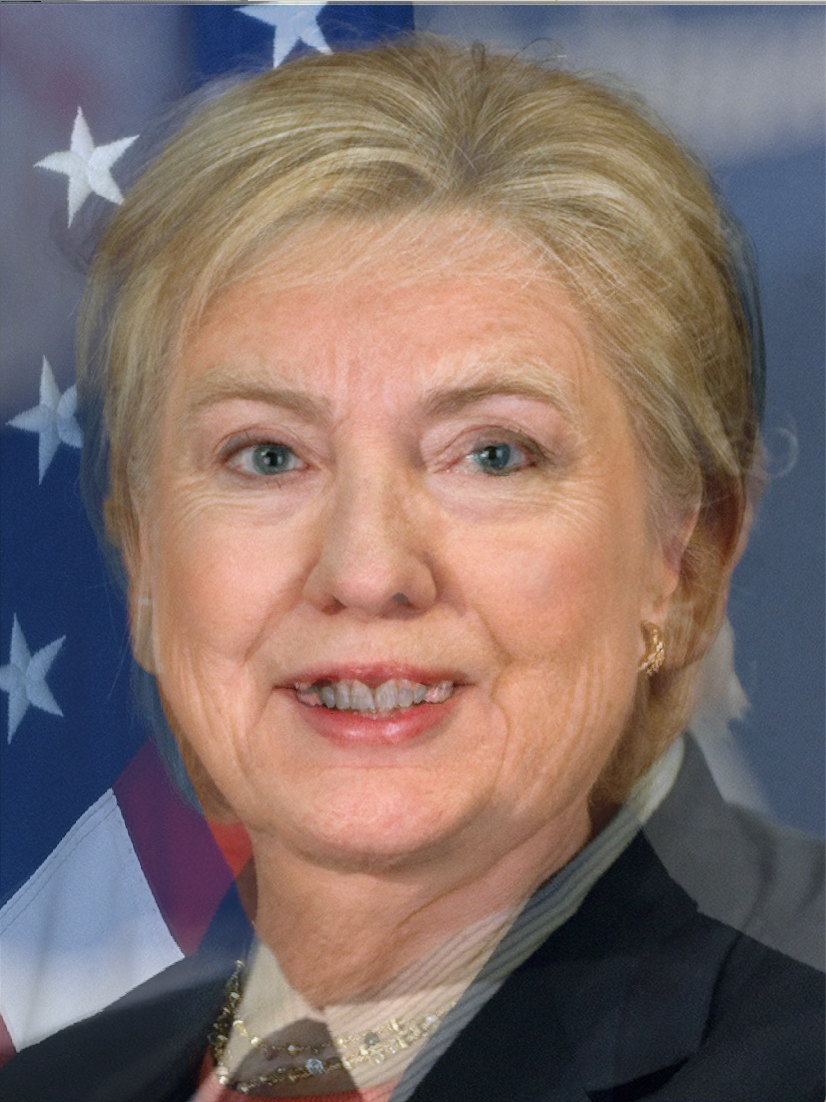
\includegraphics[width=1\columnwidth]{HT.png} 
}
\label{fig:3-4:b}
\end{minipage}
}
\hfil
\subfigure[Trump]
{
\begin{minipage}[b]{0.31\columnwidth}
\centering
\resizebox{\columnwidth}{!}{
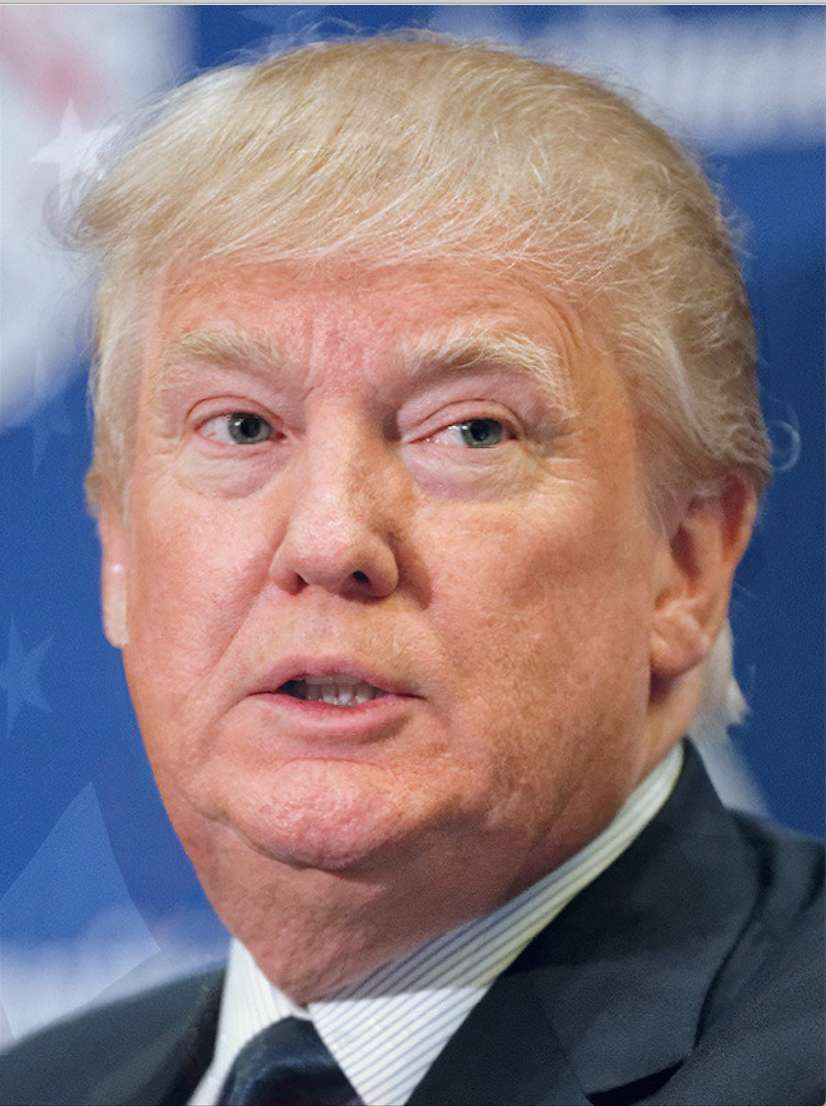
\includegraphics[width=1\columnwidth]{face_morphing/trump.png}
}
\label{fig:3-4:c}
\end{minipage}
}
\caption{Hilary+Trump}
\label{fig:3-4}
\end{figure}

\subsubsection{Trump\&Cruz}
将Trump和Cruz的人脸融合之后的效果如图\ref{fig:3-5}所示。
\begin{figure}[htp]
\centering
\subfigure[Trump]
{
\begin{minipage}[b]{0.31\columnwidth}
\centering
\resizebox{\columnwidth}{!}{
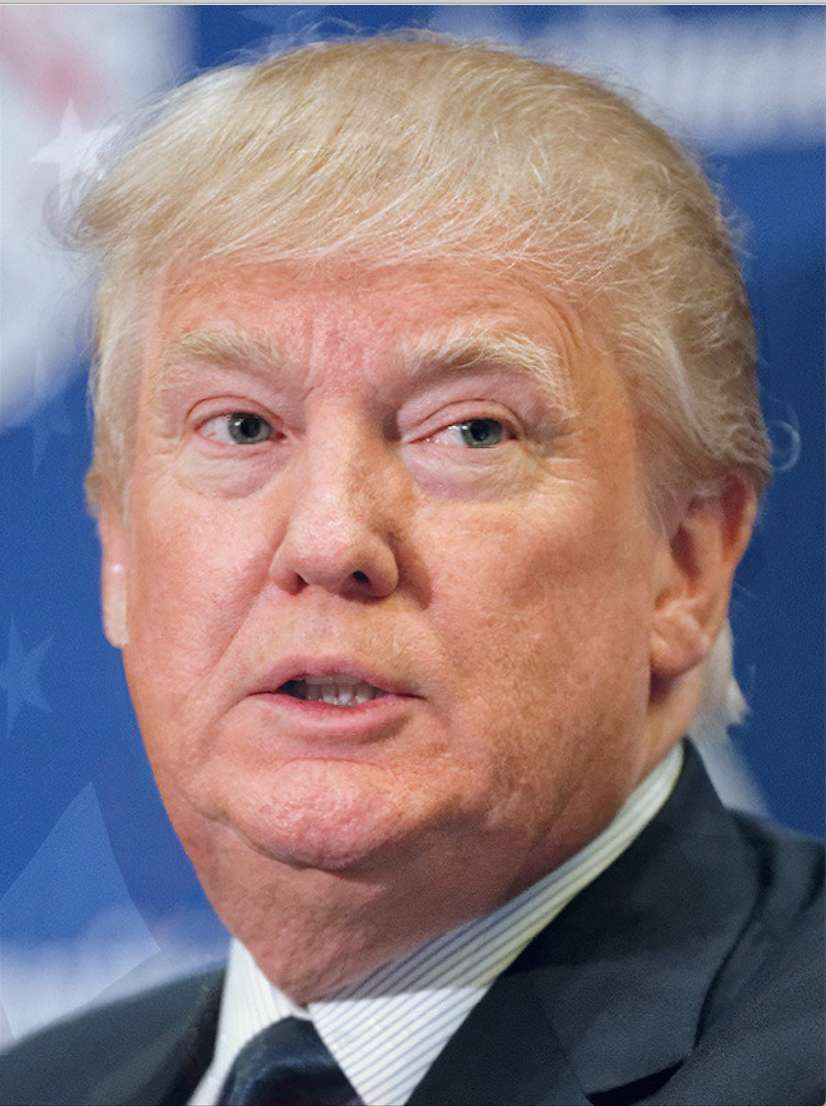
\includegraphics[width=1\columnwidth]{face_morphing/trump.png} 
}
\label{fig:3-5:a}
\end{minipage}
}
\hfil
\subfigure[0.5T+0.5C]
{
\begin{minipage}[b]{0.31\columnwidth}
\centering
\resizebox{\columnwidth}{!}{
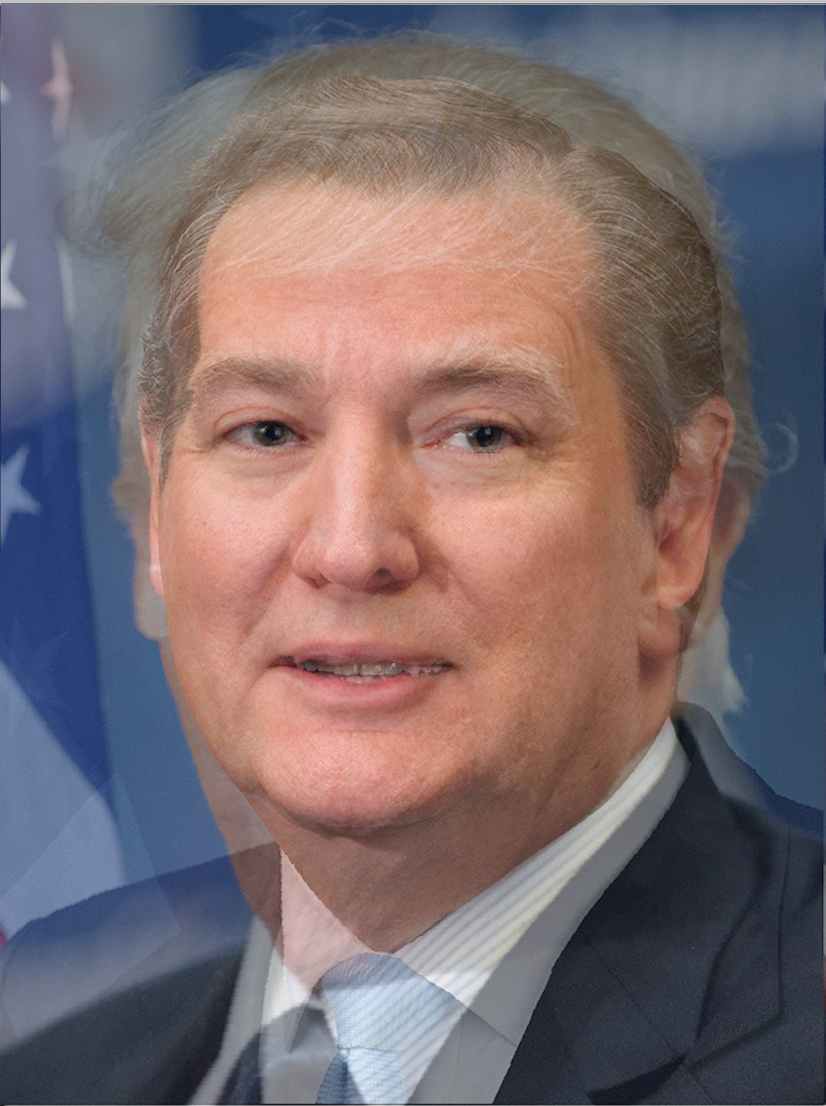
\includegraphics[width=1\columnwidth]{TC.png} 
}
\label{fig:3-5:b}
\end{minipage}
}
\hfil
\subfigure[Cruz]
{
\begin{minipage}[b]{0.31\columnwidth}
\centering
\resizebox{\columnwidth}{!}{
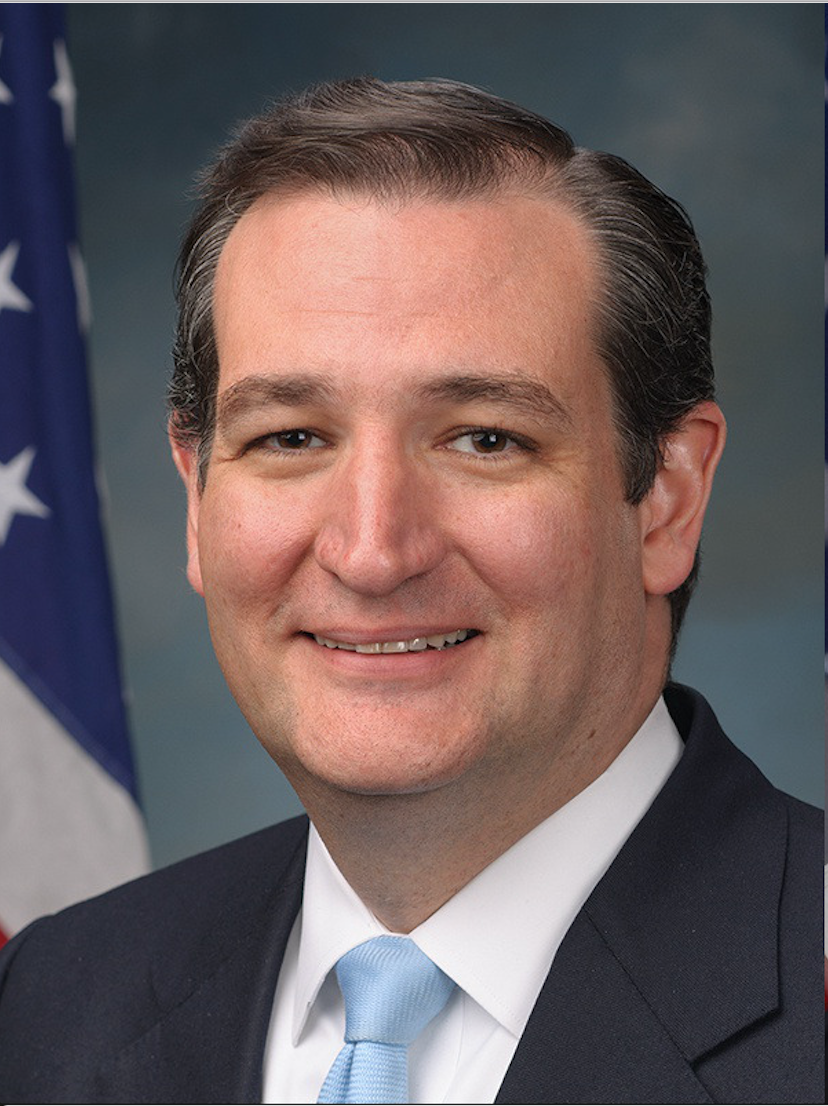
\includegraphics[width=1\columnwidth]{face_morphing/cruz.png}
}
\label{fig:3-5:c}
\end{minipage}
}
\caption{Hilary+Trump}
\label{fig:3-5}
\end{figure}

\subsubsection{Face++ API}
使用Face++ API的结果如图\ref{fig:3-6}所示。生成的图片没有ghosting,质量不错。运行时间约为两秒多。

\begin{figure}[htp]
\centering
\subfigure[0.5C+0.5H]
{
\begin{minipage}[b]{0.31\columnwidth}
\centering
\resizebox{\columnwidth}{!}{
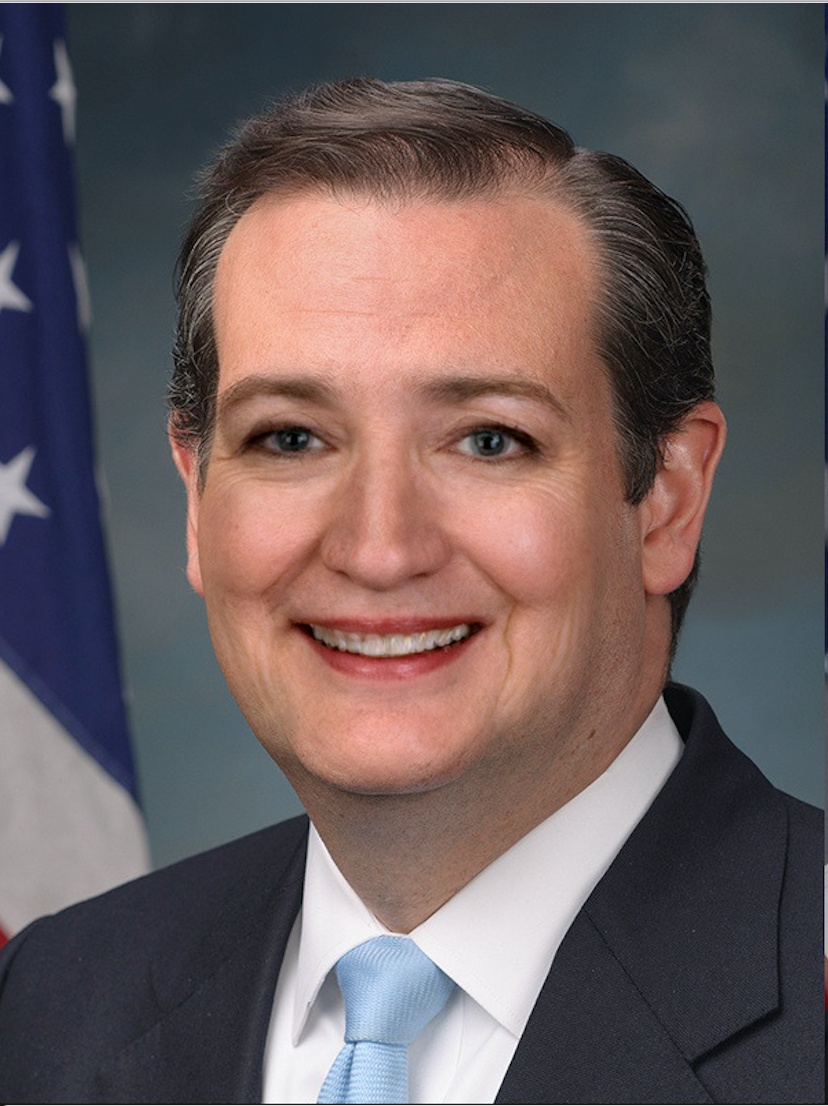
\includegraphics[width=1\columnwidth]{FCH.png}
}
\label{fig:3-5:a}
\end{minipage}
}
\hfil
\subfigure[0.5H+0.5T]
{
\begin{minipage}[b]{0.31\columnwidth}
\centering
\resizebox{\columnwidth}{!}{
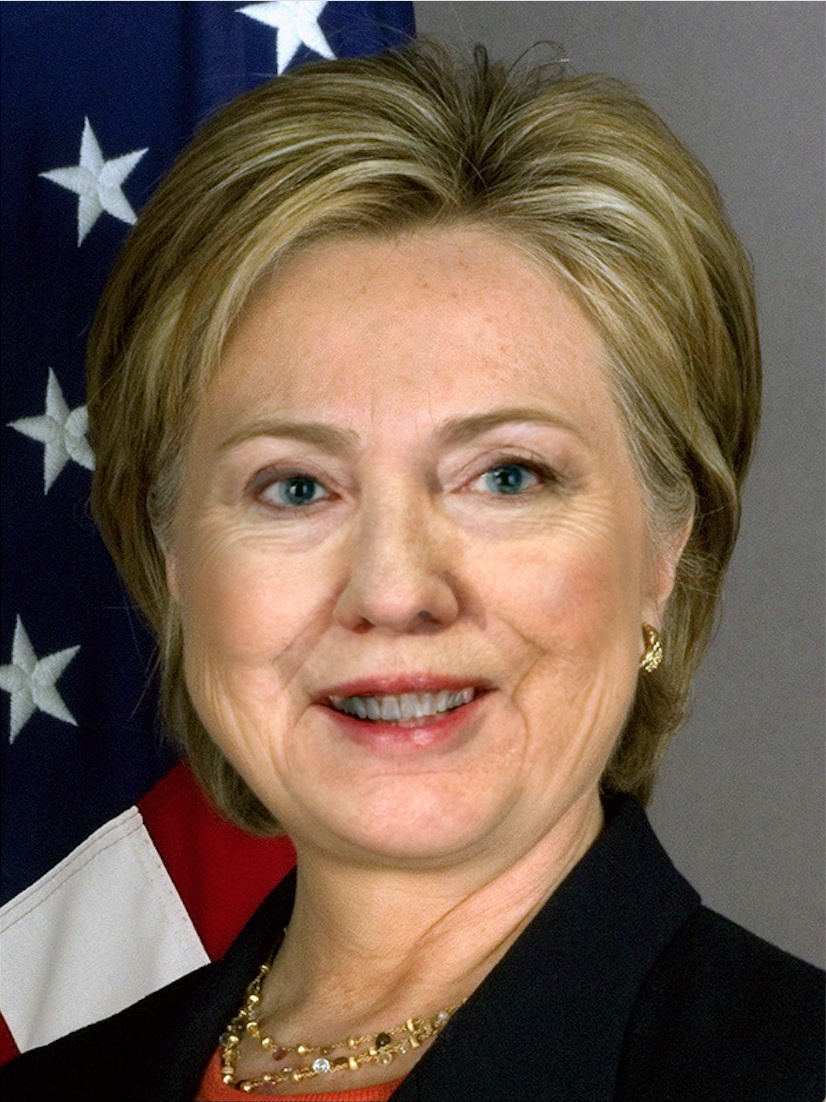
\includegraphics[width=1\columnwidth]{FHT.png} 
}
\label{fig:3-5:b}
\end{minipage}
}
\hfil
\subfigure[0.5T+0.5C]
{
\begin{minipage}[b]{0.31\columnwidth}
\centering
\resizebox{\columnwidth}{!}{
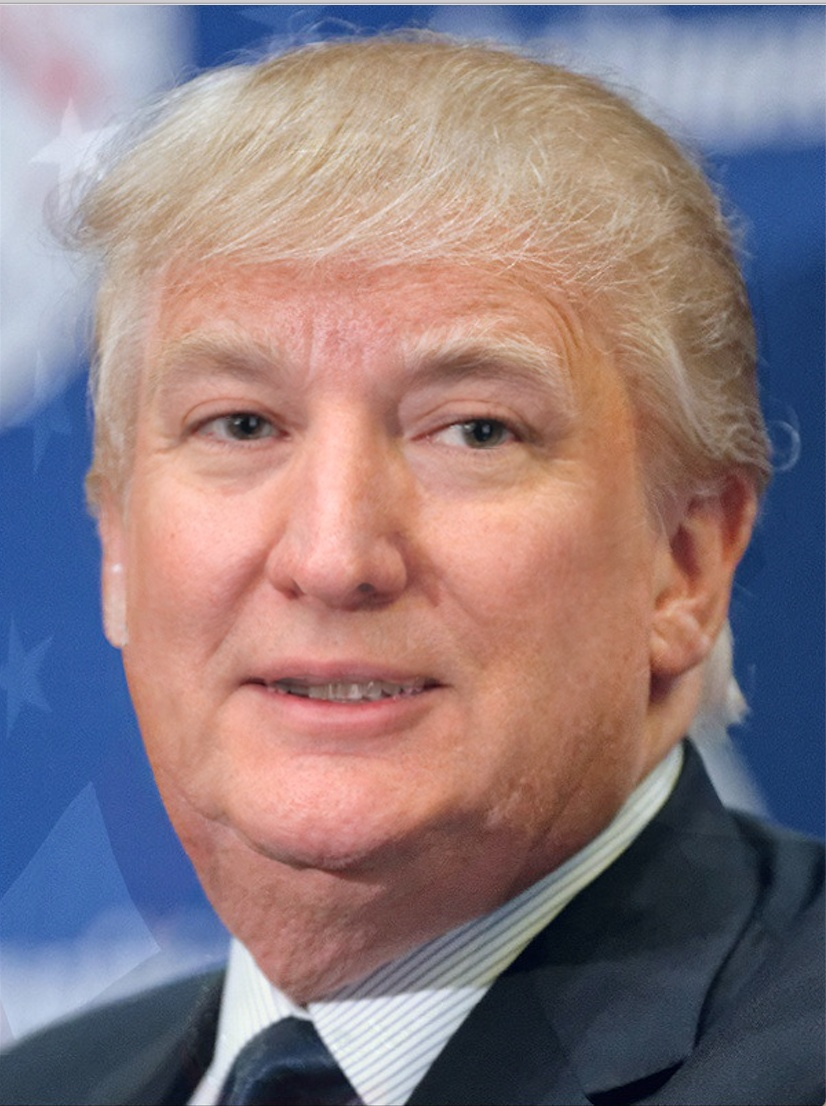
\includegraphics[width=1\columnwidth]{FTC.png}
}
\label{fig:3-5:c}
\end{minipage}
}
\hfil
\subfigure[0.5H+0.5C]
{
\begin{minipage}[b]{0.31\columnwidth}
\centering
\resizebox{\columnwidth}{!}{
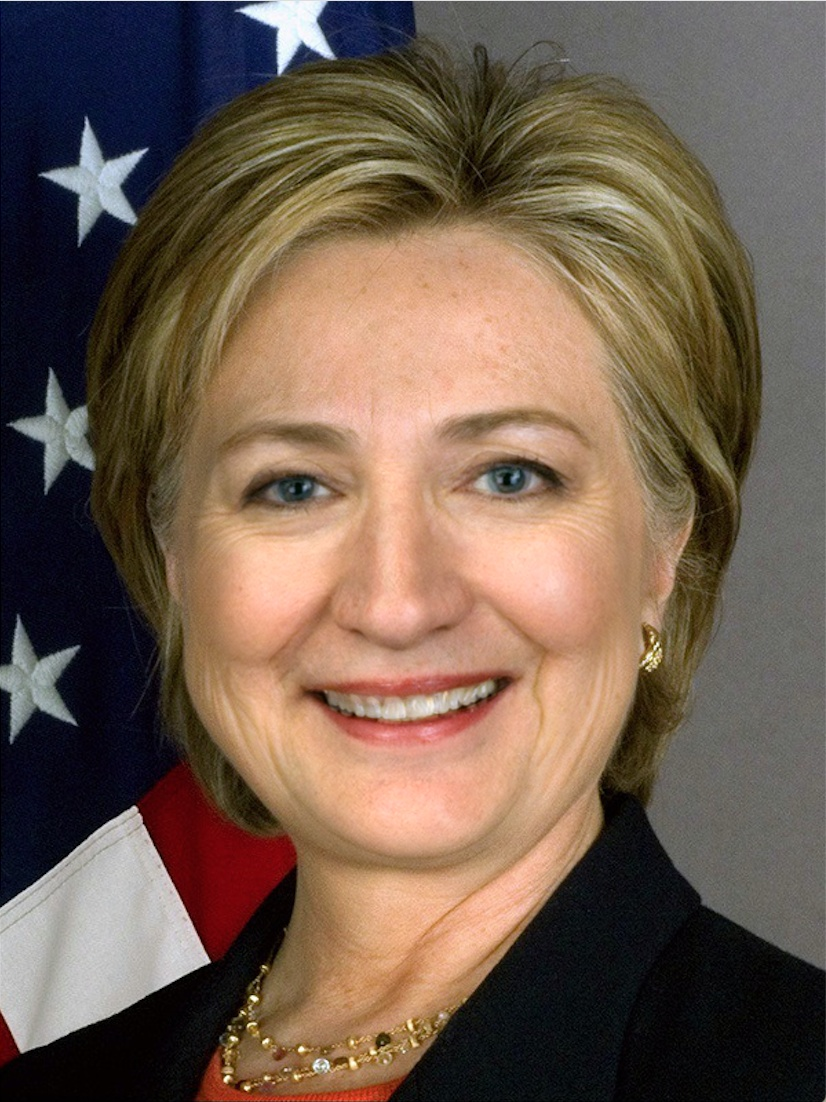
\includegraphics[width=1\columnwidth]{FHC.png}
}
\label{fig:3-5:d}
\end{minipage}
}
\hfil
\subfigure[0.5T+0.5H]
{
\begin{minipage}[b]{0.31\columnwidth}
\centering
\resizebox{\columnwidth}{!}{
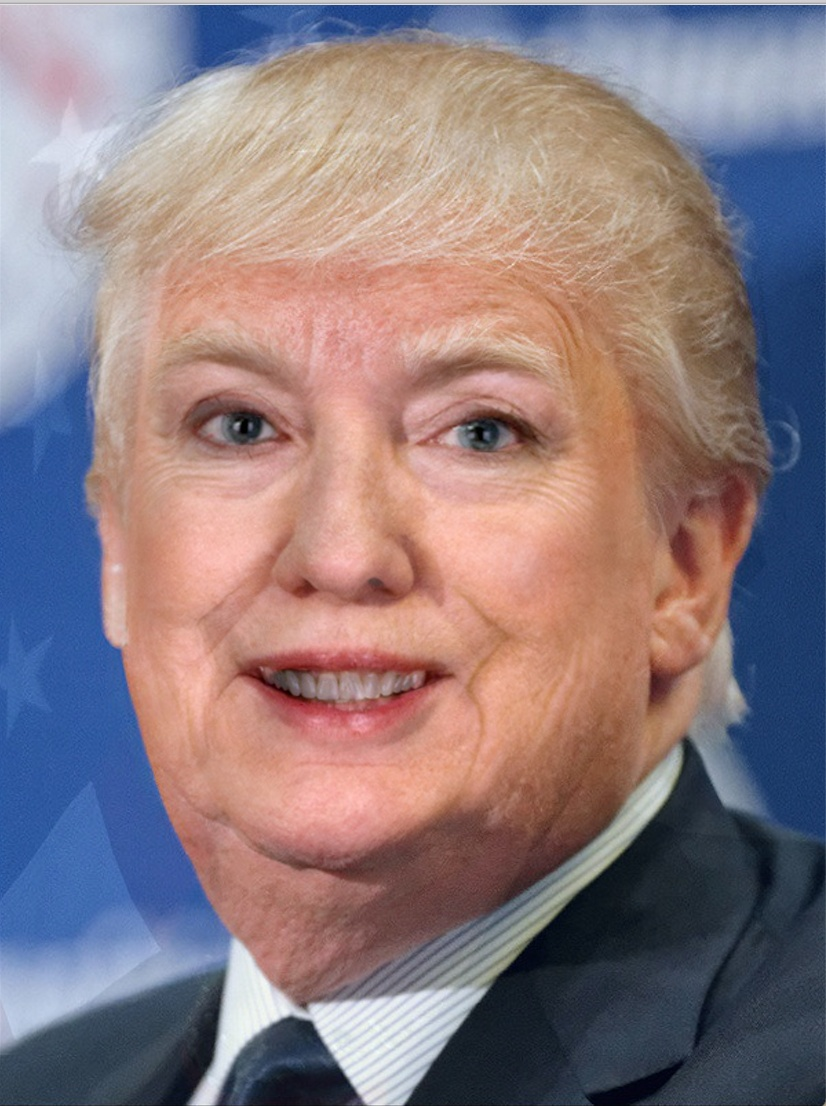
\includegraphics[width=1\columnwidth]{FTH.png} 
}
\label{fig:3-5:e}
\end{minipage}
}
\hfil
\subfigure[0.5C+0.5T]
{
\begin{minipage}[b]{0.31\columnwidth}
\centering
\resizebox{\columnwidth}{!}{
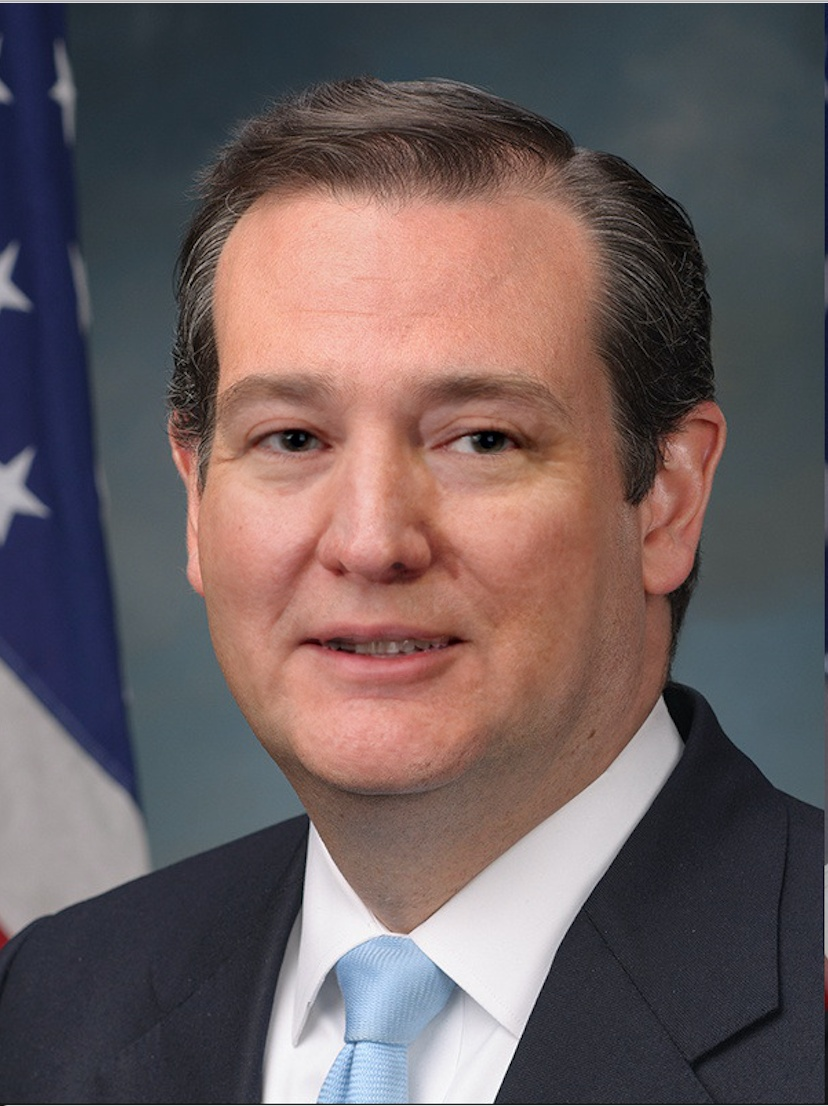
\includegraphics[width=1\columnwidth]{FCT.png}
}
\label{fig:3-5:f}
\end{minipage}
}
\caption{Face++ API result}
\label{fig:3-5}
\end{figure}


\newpage 
\bibliography{report.bib}{}
\bibliographystyle{plain}
\end{document}
